%! TEX root = ../dissertation_gurecky.tex

%-----------------------------------------------------------------------------%
\subsection{Copula}

A copula is a function which relates marginal probability distributions to a multidimensional joint distribution.  Copula provide a flexible alternative to multidimensional Gaussian based models.  Copula are utilized in this work because of their ability to capture non-Gaussian dependence structure between two or more correlated random variables, for instance temperature and the TKE at a given point on a rod's surface.  Furthermore, Sklar's theorem is used in this work in order to decompose joint distributions into a product of uni-variate marginal distributions and a copula function.  In this section, Sklar's theorem is provided along with examples of copula functions
and techniques to draw samples from them. 

The product rule of probability is shown in equation \ref{eq:prod_prob}.  To clarify notation used in this section: The comma denotes the conjunction ``and'' and the bar, $|$, is read ``given''.
\begin{equation}
P(x, y) = P(x) P(y | x)
\label{eq:prod_prob}
\end{equation}

The marginal distribution of a bivariate joint distribution $f(x, y)$ is given by equation \ref{eq:marg}.  The marginalization process is analogous to projecting the entire joint density onto a single axis.
\begin{equation}
f(x) = \int f(y) f(x|y) dy
\label{eq:marg}
\end{equation}

The cumulative density function, $F$ is defined as:
\begin{align*} 
F &= \mathbf{P}[X < x] = \int_{-\infty}^x f(x)dx \\
\end{align*}

A joint $d$ dimensional cumulative distribution is given by equation \ref{eq:joint_cdf}.
\begin{equation}
H(x_1, ... x_d) = \mathbf P[X_1 \leq x_1, ... X_d \leq x_d]
\label{eq:joint_cdf}
\end{equation}
Where $X_1, ... X_d$ are random variables.

The process of decomposing a multivariate distribution into uni-variate marginal
distributions and an object which describes their conditional dependence was
formalized by Sklar \cite{Sklar1959}.  Shown in equation \ref{eq:sklar1},  Sklar's Theorem
defines a \emph{copula} cumulative density function, $C$.
\index{Sklar's Thorem}

\begin{equation}
C(F_1(x_1), ... F_d(x_d)) = H(x_1, ... x_d)
\label{eq:sklar1}
\end{equation}
If $F_1, .. F_d$ are continuous, then $C$ is unique.  Conversely, if $C$ is a copula and $F_1, .. F_d$ are smooth cumulative destiny functions then the function $H$ is a joint cumulative distribution with margins $F_1, ... F_d$.  A proof is provided in Nelsen's introductory copula text \cite{Nelsen2006}.

Sklar also showed that the joint probability distribution, $h(x_1, ... x_d)$, can be computed from
constituent marginalized univariate distributions and the copula density, $c$.
\begin{equation}
h(x_1,\dots x_d)= c(F_1(x_1),\dots F_d(x_d))\cdot f_1(x_1)\cdot\dots\cdot f_d(x_d)
\label{eq:sklar2}
\end{equation}

For brevity, let $u_1, .. u_d$ represent samples from their CDFs as follows:
\begin{align*} u_1 &= F_1(x_1) \\ u_d &= F_d(x_d) \\ u &\in
[0, 1]
\end{align*}

Where the joint density of the copula, $c$, is given by equation \ref{eq:cop_pdf}:
\begin{equation}
c(u_1, ... u_d) = \frac{\partial C(u_1, ... u_d)}{\partial u_1 ... \partial u_d}
\label{eq:cop_pdf}
\end{equation}

Sklar's theorem enables one to construct
models for the margins separately from a model of the dependence structure.
When combined, the margins and the copula 
specify a multivariate probability density function.
Compared to rudimentary approaches based on covariance matrix dependence model,
a copula based approach can treat skewed dependence structures in which the
strength of dependence is allowed to vary depending on location in the parameter space.

\section*{Sampling Copula}
\label{sec:sampling_copula}

For simplicity, this section demonstrates how to draw correlated samples from bivariate copula.
Sampling from a bivariate copula is achieved by first defining a conditional distribution function and then applying the inverse probability integral transform.
Let $h$ represent the conditional distribution of $u_1$ given all other random variables $\{u_2, ... u_d\}$.  In the two dimensional case $h$ is given by equation \ref{eq:cop_h} \cite{Nelsen2006}:
\index{Copula!Sampling}

\begin{equation}
h(u_1 | u_2) = \frac{\partial C(u_1, u_2)}{\partial u_2}
\label{eq:cop_h}
\end{equation}

If the distribution $h$ is smooth and monotonic the inverse $h^{-1}$ exists.  For a bivariate Gaussian copula with a shape parameter $\theta_c=0.7$ the conditional distribution functions are shown in figures \ref{fig:gauss_h} and \ref{fig:gauss_hinv} for several values of the conditioning variable ($u_2$).  

\begin{figure}[!htbp]
	\centering
	\begin{minipage}{.45\textwidth}
		%
		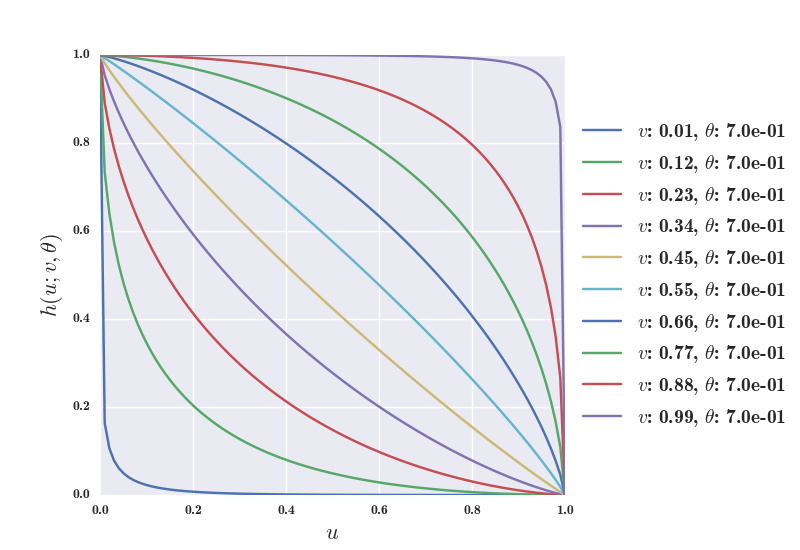
\includegraphics[width=7cm]{images/t_h_dist.png}
		\caption{The conditional $h$ \\ function vs. value of the \\ conditioning variable $u_2$ \\ for a Gaussian copula with $\theta_c=0.7$.}
		\label{fig:gauss_h}
	\end{minipage}%
	\begin{minipage}{.45\textwidth}
		%
		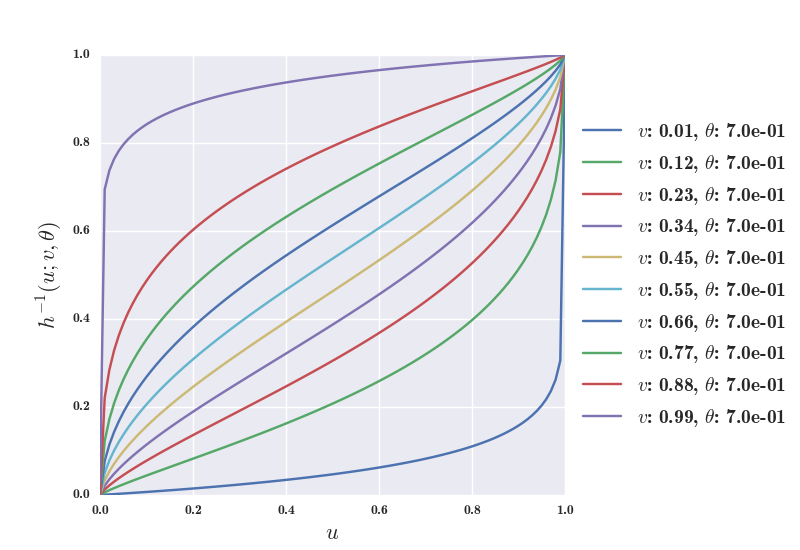
\includegraphics[width=7cm]{images/t_hinv_dist.png}
		\caption{$h^{-1}$ vs. value of the conditioning variable $u_2$ for a Gaussian copula with $\theta_c=0.7$.\\}
		\label{fig:gauss_hinv}
	\end{minipage}
\end{figure}

Computing the inverse analytically is oftentimes not possible for some classes of copula and therefore, the more general method shown in equation \ref{eq:h_inv_sample} is used.
A random vector of length $N$ is drawn from the uniform distribution $\in [0, 1]$:  $\{\mathbf U_2\}$.  For each sample, $u_{2_i}$ in $\{\mathbf U_2\}$ the 1-D line search problem given in equation \ref{eq:h_inv_sample} is solved.  This produces a sample vector of length $N$: $\{\mathbf U_1\}$.

\begin{equation}
u_{1_i} = \mathrm{argmin}_{u_1} \left[ h(u_1|u_{2_i}) - u_{2_i} \right],\ \mathrm{with}\ 0 < u_1 < 1
\label{eq:h_inv_sample}
\end{equation}

The resulting correlated sample vectors $\{\mathbf U_1, \mathbf U_2\} \in [0,1]^2$ are distributed according to the copula, $c$, and have uniform margins.  An example of random samples drawn from a Gaussian copula are shown in figure \ref{fig:gauss_samples}.  The smooth Gaussian copula PDF is provided in figure \ref{fig:gauss_pdf}.

\begin{figure}[!htbp]
	\centering
	\begin{minipage}{.45\textwidth}
		%
		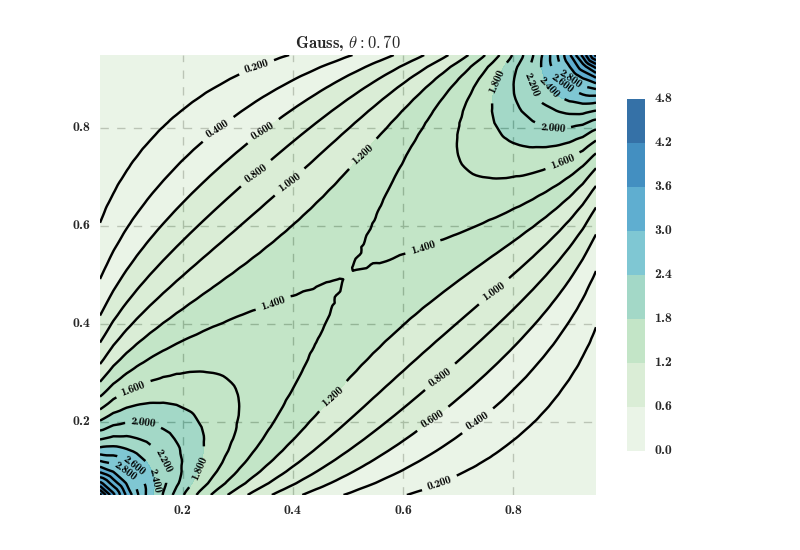
\includegraphics[width=9.2cm]{images/gauss_copula_pdf.png}
		\caption{Gaussian copula density\\ with $\theta_c=0.7$.}
		\label{fig:gauss_pdf}
	\end{minipage}%
	\begin{minipage}{.45\textwidth}
		%
		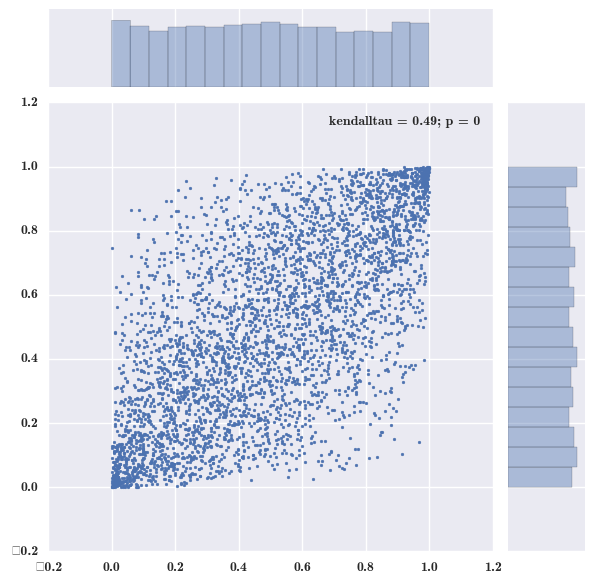
\includegraphics[width=7cm]{images/gauss_samples.png}
		\caption{Samples drawn from Gaussian copula\\ with $\theta_c=0.7$.}
		\label{fig:gauss_samples}
	\end{minipage}
\end{figure}

To apply arbitrary margins $F_1$ and $F_2$ we employ, again, the inverse probability transform. 
Correlated samples are then drawn according to:
\begin{eqnarray}
\mathbf X = & F_1^{-1}(\mathbf U_1) \\
\mathbf Y = & F_2^{-1}(\mathbf U_2)
\end{eqnarray}
The sample vectors $\{\mathbf X, \mathbf Y\}$ are distributed according to the joint density, $C(F_1, F_2)$.  An example bivariate sample set with exponentially distributed margins and a Gaussian copula is shown in figure \ref{fig:gauss_samples_scaled}.  In the example figure both margins follow an exponential distribution given by $f(x)=\lambda e^{-\lambda x}$ with $\lambda=2\mathrm{E-}3$.

\begin{figure}[!htbp]
	\centering
	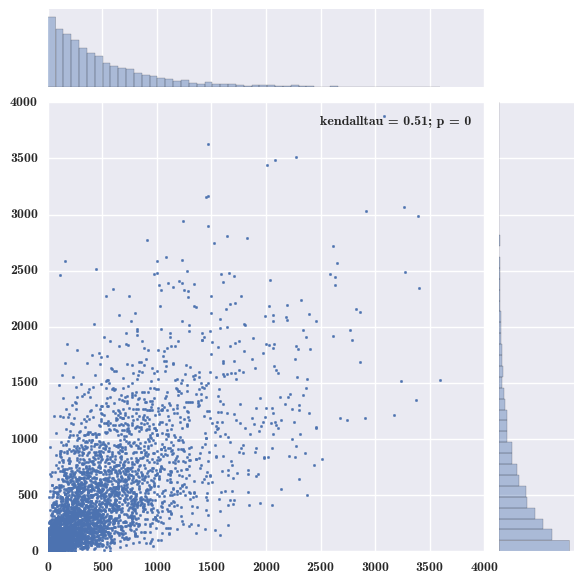
\includegraphics[width=9cm]{images/gauss_samples_scaled.png}
	\caption{Samples drawn from Gaussian copula with exponential margins.}
	\label{fig:gauss_samples_scaled}
\end{figure}


\section*{Copula Families}

A wide range of copula functions are available in the literature.  In order to satisfy the definition of a copula several criteria must be met:
\begin{enumerate}
	\item Must integrate to one on $[0, 1]^n$
	\item Must have uniform marginal distributions (as shown in figure \ref{fig:gauss_samples}).
	\item When one argument to the joint copula CDF is zero, the CFD is zero:
	\begin{equation}
	C(u_1, u_2, ... 0, ... u_d) = 0
	\end{equation}
	\item When one argument to the joint copula CDF is $u\in[0,1]$ and all other arguments are one, the CFD takes a value equal to $u$:
	\begin{equation}
	C(1, 1, ... u, ... 1) = u
	\end{equation}
\end{enumerate}

Examples of valid copula are given in figure \ref{fig:montage_cop}.  A wide range of skewed dependence structures can be represented by considering only a few copula families.  Each copula can be rotated to accommodate both positive or negative dependence.

\begin{figure}[!htbp]
	\centering
	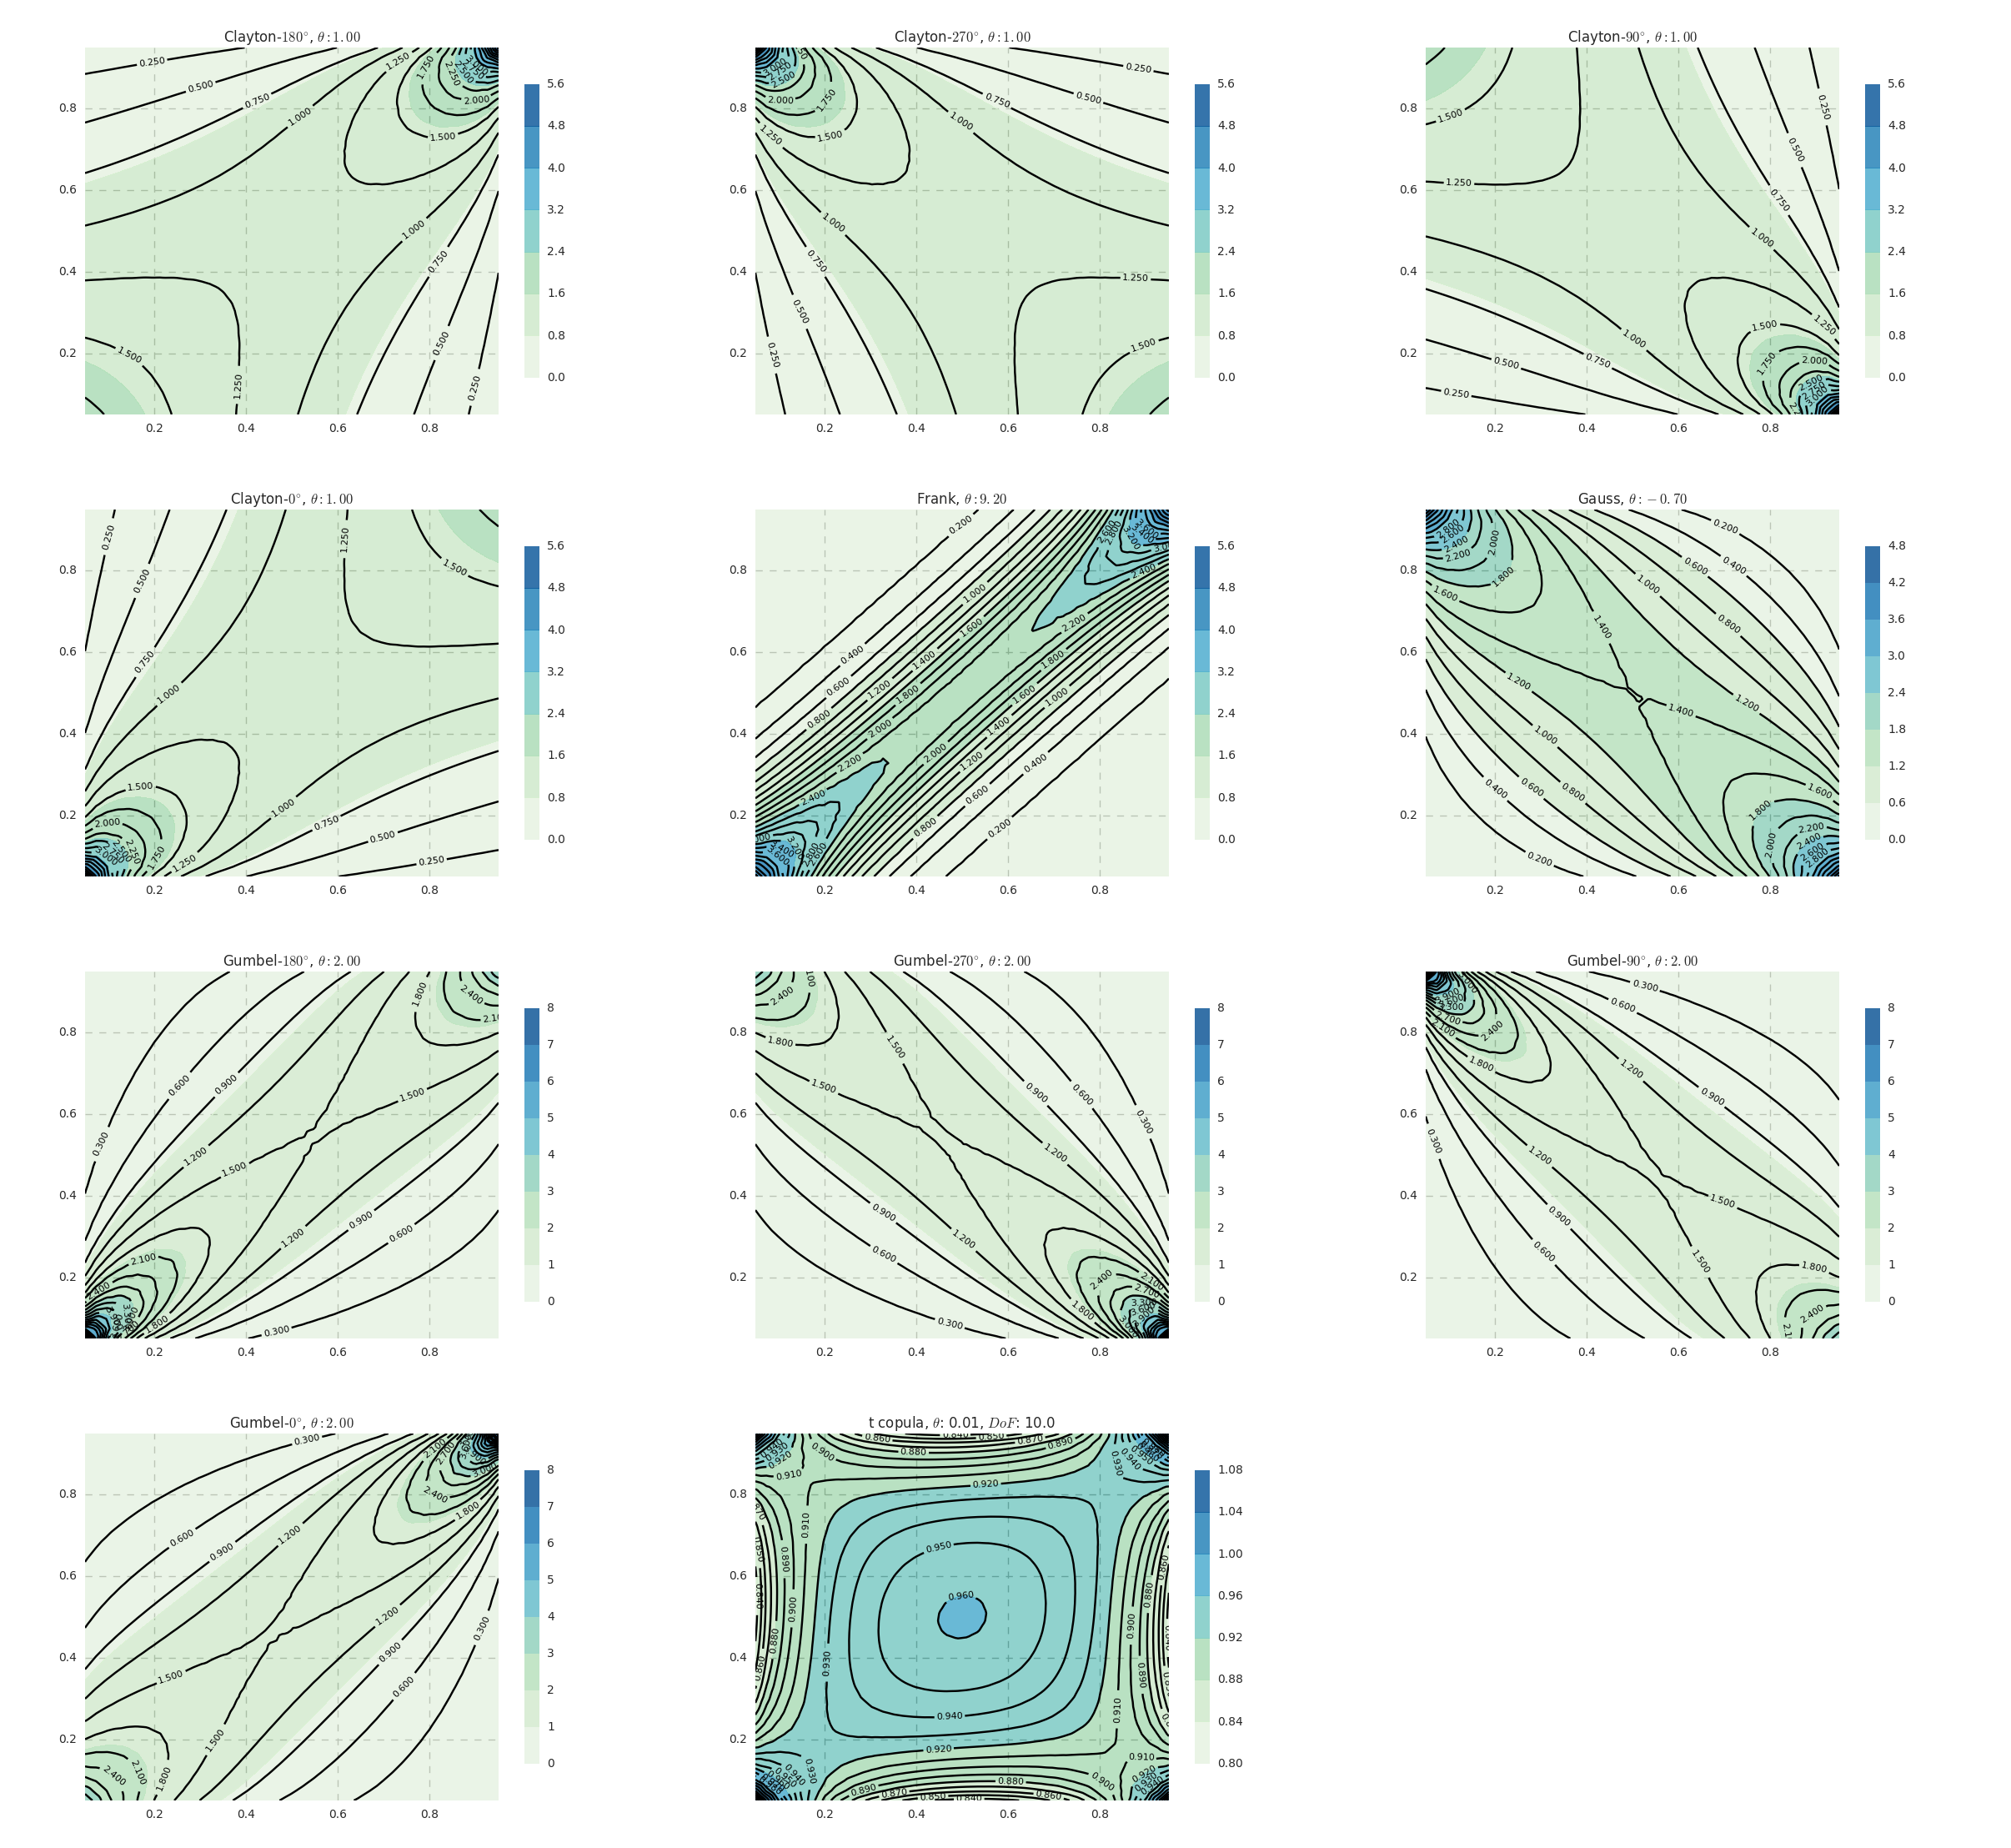
\includegraphics[width=18cm]{images/montage_copula_pdf.png}
	\caption{Examples of bivariate copula PDFs.}
	\label{fig:montage_cop}
\end{figure}

\subsection{Fitting Copula}
\label{sec:fitting_copula}

Fitting copula to empirical data can be carried out by the method of maximum likelihood (ML).  Consider the bivariate case where $N$ sample pairs, $\{w_i, v_i\}_{i\in [ 1,N ] }$  are known. The likelihood function for a copula is given by equation \ref{eq:lik}.  The likelihood is a function of the distribution parameter $\theta_c$ with the data, $\{\mathbf w,\mathbf v \}$, held fixed. When integrated over all possible parameter values the integrated result does not necessarily take on a value of unity and therefore cannot be strictly interpreted as a probability density. Each constituent factor in the likelihood function can be interpreted as the relative likelihood that the sample pair $\{w_i, v_i\}$ arose from the copula density function with parameter $\theta_c$.
\index{Copula!Fitting}

\begin{equation}
    \mathcal{L}(\theta_c;\mathbf w,\mathbf v)= \prod_{i=1}^N c(w_i, v_i|\theta_c)
\label{eq:lik}
\end{equation}

Where $\theta_c$ is the free copula shape parameter.
Typically the negative log-likelihood, $-\mathrm{ln}\mathcal{L}$, is used in when performing ML estimation of a distribution parameter since the problem is typically cast in terms of a minimization problem.  
\begin{equation}
\hat \theta_{c,ML} = \mathrm{argmin}_{\theta_c}[-\mathrm{ln}\mathcal{L}(\theta_{c} ; \mathbf w, \mathbf v)]
\label{eq:nlog_lik}
\end{equation}
\index{Maximum Likelihood}

To minimize the negative log likelihood in equation \ref{eq:nlog_lik}  one computes the partial derivative with respect to $\theta_c$ and finds the value $\hat \theta_{c,ML}$ for which this expression reaches zero.  This can be carried out by Newton's method.  If the partial derivatives of the copula's negative log likelihood are impossible to compute analytically one can estimate them by finite difference.

In order to determine which copula family best represents the data, an arsenal of statistical tests can be applied to select the copula which best fits the data.  Here, we consider two methods:  (1) Comparing Akaike information criterion (AIC) and (2) graphically comparing each fitted copula.  

The AIC is computed by equation \ref{eq:cop_aic}.
\begin{equation}
\mathrm{AIC} = 2k - 2\mathrm{ln}(\mathcal{L})
\label{eq:cop_aic}
\end{equation}
Where $k$ is the number of free parameters in the model.  The AIC penalizes models with larger numbers of parameters. 
Automated copula selection is achieved by selecting the copula that obtains the lowest AIC score.

A graphical method of copula selection was proposed by Barbe et. al. (1996) \cite{Barbe1996}.  In this method each trial copula's Kendall's function, $K_c(t)$ is plotted against an empirical estimate of this function, $\hat K_c$.  Given $d$ random variables $\mathbf U=\{U_1, ... U_d\}$ distributed according to some $d$ dimensional copula, $C$, Kendall's function is given by \ref{eq:Kc} \cite{Joe2015}.
\begin{equation}
K_c(t; C) = \mathrm P \left[C(\mathbf U) \leq t; \mathbf{U} \sim\ C\right]
\label{eq:Kc}
\end{equation}

\begin{figure}[!htbp]
	\centering
	\begin{minipage}{.45\textwidth}
		%
		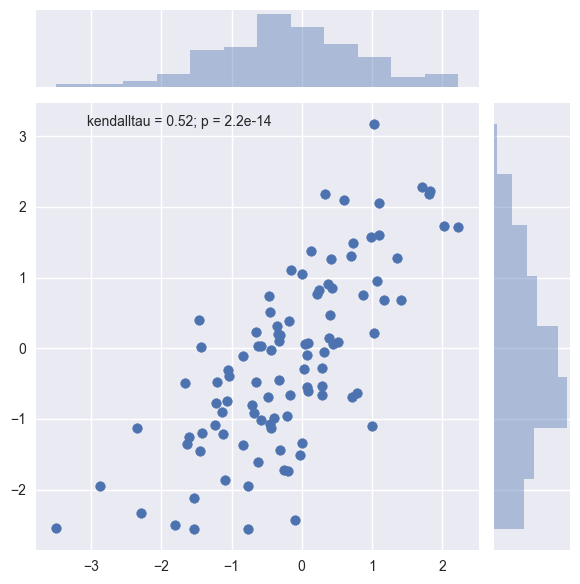
\includegraphics[width=6.5cm]{images/original_stocks.png}
		\caption{Ficticious bivariate \\ data set.}
		\label{fig:biv_data_ex}
	\end{minipage}%
	\begin{minipage}{.45\textwidth}
		%
		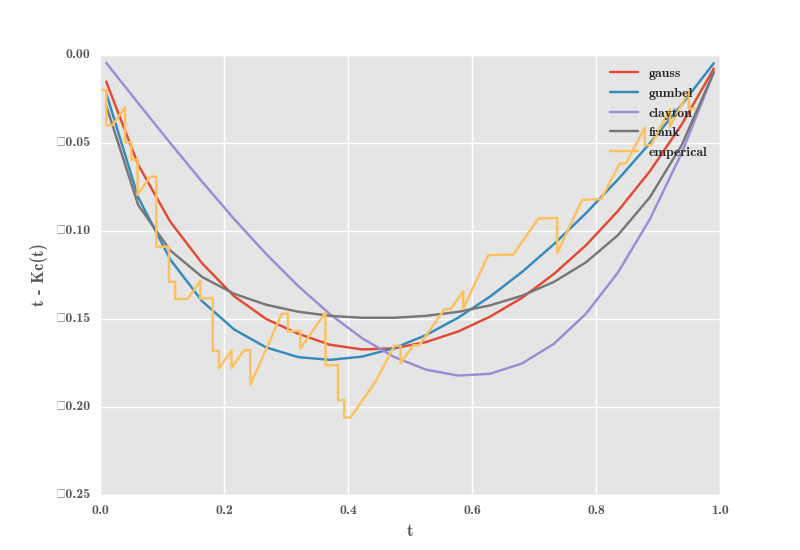
\includegraphics[width=9cm]{images/ktau_function_plot1.png}
		\caption{Graphical comparison of  \\ Kendall's distribution for \\ several fitted copula.}
		\label{fig:kc_fn_compare}
	\end{minipage}
\end{figure}
For example, by graphical inspection of figure \ref{fig:kc_fn_compare}, the Gumbel copula is the best fit to the original data set.  This visual process can be automated by computing and comparing $||\hat K_c(t) - K_c(t)||$ for each trial copula.

\subsection*{Kendall's Tau}

Kendall's tau is a measure of concordance.  Consider two correlated and uniformly distributed random variables, $X, Y$.
%  If a rank $x_{(i)}$ is drawn for the first variable, the likelihood that you will also have drawn the rank $y_{(i)}$ of the second to be at least as great as the first is proportional to Kendall's tau.  More precisely, 
Let $(X_1, Y_1)$ and $(X_2, Y_2)$ be identically distributed random vectors from some joint cumulative distribution so that individual samples from $X\ and\ Y$ will take on values in $[0,1]$, then Kendall's tau is given by equation \ref{eq:ktau} \cite{Nelsen2006}.  
\index{Kendall's Tau}

\begin{equation}
\rho_\tau = P[(X_1 - X_2)(Y_1-Y_2)>0] - P[(X_1 - X_2)(Y_1 - Y_2)<0]
\label{eq:ktau}
\end{equation}

In the case of Archimedean copula, $\rho_\tau$ is directly related to the copula's parameter, $\theta_c$.
Equation \ref{eq:tauar} relates an Archimedean copula's parameter to $\rho_\tau$.  This is useful since if one can estimate $\rho_\tau$ from the empirical data and the copula type is known, one can quickly compute the copula's shape parameter without resorting to the method of ML.

\begin{equation}
\rho_\tau = 1 + 4 \int_0^1 \frac{\varphi(\theta_c,t)}{\varphi'(\theta_c, t)}dt
\label{eq:tauar}
\end{equation}
Where $\varphi(t)$ is the copula's generator function and $\varphi'(t)$ is the first derivative of the generator function with respect to $t$. A list of copula generator functions may be found in introductory copula texts \cite{Nelsen2006}.

%\subsection*{Archimedean Copula}

%Archimedean copula are defined by the relationship.

%Where $\psi$ is a monotonically decreasing and convex function.

%A simplification can be made when fitting Archimedean copula since there is a one-to-one relationshipt between $\rho_\tau$ and the copula's shape parameter, $\theta_c$.

